\documentclass[11pt,xcolor=dvipsnames,aspectratio=169]{beamer}

\mode<presentation>
{
  \useinnertheme{circles} 
  \usecolortheme[named=Black]{structure} 
  \setbeamertemplate{navigation symbols}{}
  \setbeamertemplate{footline}[page number]
  \setbeamercovered{transparent}
}

\usepackage{physcomm}

%\usepackage{adjustbox}
\usepackage[export]{adjustbox}
\usepackage{graphicx}
\usepackage{colortbl}
\usepackage{pifont}
\usepackage{amsmath}
\usepackage{scrdate,scrtime}
\usepackage{subfig}
\usepackage{verbatim}
\usepackage{booktabs}
\usepackage{rotating}
\usepackage{xspace}
\usepackage{xcolor}
\usepackage{bm}
\usepackage{pdfpages}
\usepackage{enumerate}
\usepackage{amsmath}
\usepackage{xspace}
\usepackage{ifthen}
 
%-----------------------------------------------------------------------
% custom colors 
\definecolor{EDBRed}{RGB}{220,20,60} 
\definecolor{EDBDarkBlue}{RGB}{0,0,160}
\definecolor{EDBBlue}{RGB}{0,135,189}
\definecolor{EDBGray}{RGB}{211,211,211}

%-----------------------------------------------------------------------
% text boxes 
\usepackage{tcolorbox}
%\usepackage{mdframed}

% 1- Block title (background and text)
\setbeamercolor{block title}{bg=EDBBlue!60, fg=black}
% 2- Block body (background)
\setbeamercolor{block body}{bg=EDBBlue!60}

\setbeamercolor{block title alerted}{fg=white, bg=orange}
% 2- Block body (background)
\setbeamercolor{block body alerted}{bg=orange!25}

% 1- Block title (background and text)
\setbeamercolor{block title example}{fg=white, bg=teal}
% 2- Block body (background and text)
\setbeamercolor{block body example}{bg=EDBBlue!60}

% arrows between color boxes
\usepackage{tikz}
\usetikzlibrary{arrows.meta, % for arrows style
                positioning  % for positioning of boxes
               }

%-----------------------------------------------------------------------
% backup 
\newcommand{\backupbegin}{
   \newcounter{framenumberappendix}
   \setcounter{framenumberappendix}{\value{framenumber}}
    \setbeamertemplate{footline}{
   \leavevmode%
   \hbox{%
   \begin{beamercolorbox}[wd=1.00\paperwidth,ht=0.01ex,dp=1ex,right]{} 
     {\normalsize \insertframenumber{}} \hspace{0.065\textwidth}
   \end{beamercolorbox}
   }%
   \vskip0pt%
 }
}

\newcommand{\backupend}{
   \addtocounter{framenumberappendix}{-\value{framenumber}}
   \addtocounter{framenumber}{\value{framenumberappendix}} 
}

% -----------------------------------------------------------------------
% slide layout & footnotes
\setbeamertemplate{frametitle}{ 
%\begin{centering} 
\vspace{0.03\paperheight}
{\huge \insertframetitle }
\vspace{0.01\paperheight}
\par 
%\end{centering} 
}


%\setbeamertemplate{footline}[text line]{%
%\parbox{\linewidth}{\small \vspace*{-10pt} \ \hfill \ \insertpagenumber / \inserttotalframenumber}}

\setbeamertemplate{footline}[text line]{%
\parbox{\linewidth}{\small \vspace*{-10pt} \ \hfill \ \insertframenumber / \inserttotalframenumber}}

\let\footnoterule\relax

\newcommand\blfootnote[1]{%
  \begingroup
  \renewcommand\thefootnote{}\footnote{\hspace{-30pt}\textcolor{Gray}{\tiny #1}}%
  \addtocounter{footnote}{-1}%
  \endgroup
}

% -----------------------------------------------------------------------
% itemize margins
\setlength{\leftmargini}{0.025\linewidth}
\setlength{\leftmarginii}{0.021\linewidth}

% sub-item size:
\setbeamerfont{itemize/enumerate subbody}{size=\normalsize} %to set the body size
%\setbeamertemplate{itemize subitem}{\normalsize\raise1.25pt\hbox{\donotcoloroutermaths$\blacktriangleright$}}  %to set the symbol size 
% -----------------------------------------------------------------------
\begin{document}

{
\usebackgroundtemplate{
\includegraphics[width=\paperwidth]{background/template_169_logos.pdf}}%
\begin{frame}[noframenumbering,plain]
  \begin{center}
    \setlength{\parskip}{0pt}
    \vspace{10pt}
    {\Huge\bf Deep Learning \& the Higgs Boson}\\[0.1\textheight]
    {\huge \bf Dr. Liza Mijovi\'c}
  \end{center}
\end{frame}
}

{
\usebackgroundtemplate{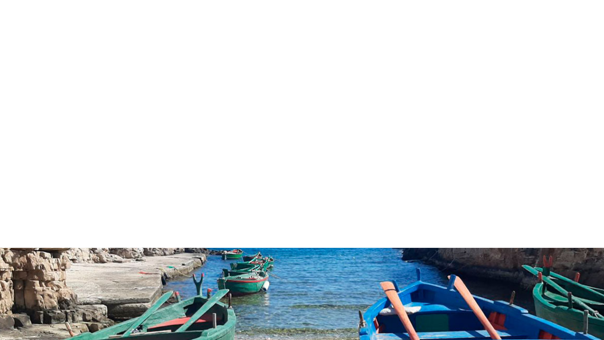
\includegraphics[width=\paperwidth]{background/template_169.pdf}}%
\begin{frame}[plain]
  \frametitle{\bf Deep Learning \& the Higgs Boson}
  \adjustbox{valign=t}{\begin{minipage}[t][0.55\textheight]{\linewidth}
      Classification with Fully Connected and Adversarial Networks.
      \vfill
      \begin{itemize}
      \item {\bf Lecture1: The Higgs boson and event classification:}\\
        - Event classification with a fully connected neural network (NN) with Keras API.\\
      \end{itemize}
      \vfill
      \begin{itemize}      
      \item {\bf Lecture2: Solving the background sculpting challenge:}\\
        - Event classification with adversarial neural network (ANN).\\
        - Hands-on knowledge of manipulating neural networks in Tensorflow.
      \end{itemize}
      \vfill
      \begin{itemize}          
      \item {\bf Lecture3: Putting it all together:}\\
        - Compare ANN classification performance to the fully connected network.
      \end{itemize}
      \vfill
\end{minipage}}
% vertical place-holder
\adjustbox{valign=t}{\begin{minipage}[t][0.35\textheight]{\linewidth} 
  \end{minipage}}
\end{frame}
}


{
\usebackgroundtemplate{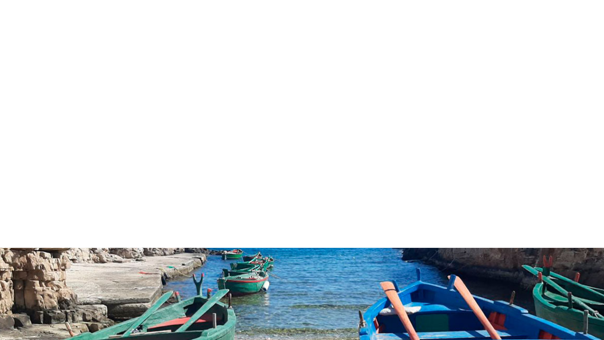
\includegraphics[width=\paperwidth]{background/template_169.pdf}}%
\begin{frame}[plain]
  \frametitle{\bf Lecture3:  Putting it all together}
  \adjustbox{valign=t}{\begin{minipage}[t][0.55\textheight]{\linewidth}
      \vfill
      \begin{itemize}
      \item {\bf Hands-on: 40'}\\
        Compare fully connected and adversarial network classification performance. 
      \end{itemize}
      \begin{itemize}
      \item {\bf Lecture2 survey discussion: 15'}
      \end{itemize}
      \begin{itemize}
      \item {\bf Lecture3 results discussion: 15'}       
      \end{itemize}
      \begin{itemize}
      \item {\bf Wrap up: CERN open data \& LHC AI challenges.}
      \end{itemize}        
      \vfill
\end{minipage}}
% vertical place-holder
\adjustbox{valign=t}{\begin{minipage}[t][0.35\textheight]{\linewidth} 
  \end{minipage}}
\end{frame}
}



\begin{frame}
  \frametitle{\bf Reminder: Our Challenge}

  \adjustbox{valign=t}{\begin{minipage}[c]{0.5\linewidth}
      \vfill
        {\bf Classification: separate}
        \begin{itemize}
        \item \textcolor{EDBRed}{Signal} with Higgs boson.
        \item \textcolor{EDBBlue}{Background} with no Higgs boson.
        \end{itemize}
        \vfill
        {\bf Approach:} 
        \begin{itemize}
        \item use synthetic data.
        \item \textcolor{EDBBlue}{Introduce no bumps in the \myy{} distribution;
            these would hamper the background estimate.}
        \end{itemize} 
      \end{minipage}}
    \adjustbox{valign=t}{\begin{minipage}[c]{0.49\linewidth}     
      \begin{figure}
        \includegraphics[width=1.00\textwidth]{figures/l1/challenge/figaux_01.pdf}
      \end{figure}
    \end{minipage}}
   \blfootnote{\scriptsize{L. Mijovi\'c, ATLAS, \href{https://arxiv.org/abs/2207.00348}{JHEP (2022)}.}}  
\end{frame}

\begin{frame}
  \frametitle{\bf Reminder: What is in the data?}
  \begin{itemize}
  \item Momenta $p$ are  4-dimensional (Lorentz) vectors.
  \item They are passed in cylindrical coordinates.
  \end{itemize}
  \begin{figure}
    \includegraphics[width=1.00\textwidth]{figures/l1/challenge/data_annot.png}
  \end{figure}
\end{frame}

\begin{frame}
  \frametitle{\bf Lecture1: fully connected network}
  \adjustbox{valign=c}{\begin{minipage}[c]{0.49\linewidth}
      Fully connected deep neural network.\\
      {\bf Inputs:}
        \begin{itemize}
        \item Features $x$: photon 4-vectors.
        \item Labels $y$: signal (1) or background (0).
        \end{itemize}
        {\bf Output:}
        \begin{itemize}
        \item discriminant: $z = p_{clf}(y|x,\theta_{clf})$.
        \end{itemize}
    \end{minipage}}
    \adjustbox{valign=c}{\begin{minipage}[c]{0.45\linewidth}     
      \begin{figure}
        \includegraphics[width=1.00\textwidth]{figures/l2/class.pdf}
      \end{figure}
    \end{minipage}}
\end{frame}

\begin{frame}
  \frametitle{\bf Lecture1: Classification Results}
  \vspace{-5pt}
      \begin{figure}
        \includegraphics[width=1.00\textwidth]{figures/l3/7.pdf}
      \end{figure}
\end{frame}

\begin{frame}
  \frametitle{\bf Lecture2: Adversarial Neural Network}
  \begin{itemize}
  \item Both networks trained simultaneously with a loss:
    $$ L = L_{clf}(\textcolor{EDBBlue}{\theta_{clf}})-\lambda L_{adv}(\textcolor{EDBBlue}{\theta_{clf}},\textcolor{EDBRed}{\theta_{adv}}) $$
  \item \textcolor{EDBBlue}{Classifier:} tries to guess event label ($y$ = signal or background).
  \item \textcolor{EDBRed}{Adversary:} tries to guess $d=\myy{}$.   
  \item Trade-off controlled by parameter $\lambda$.
  \end{itemize}
  \begin{figure}
    \includegraphics[width=1.0\textwidth]{figures/l2/and_ann.png}
  \end{figure}
  \blfootnote{Adapted from: A. Sogaard's,
    \href{https://github.com/asogaard/ep2mlf/blob/master/01-adversarial/2018-11-13_EP2MLF_AndreasSogaard.pdf}{lecture
    on adversarial NN.}}
\end{frame}


\begin{frame}
  \frametitle{\bf Hands-on work}

  {\bf Compare classification with fully connected and adversarial network.}
  \begin{itemize}
  \item Classification performance, eg ROC curve.
  \item S and B myy distribution, for high discriminant scores (events likely to
    be S). Does ANN reduce bumps in the background \myy{} spectrum? 
  \end{itemize}
  {\bf Further suggestions:}
  \begin{itemize}
  \item Any discriminant scores, for which ANN background \myy{} is bumpy?
  \item Train/validation loss curves as expected?
  \end{itemize}
  {\bf Where is the data:} 
  \begin{itemize}
  \item (1) Yesterday: you ran code/final/ann\_classification.ipynb over 200k events
  \item (2) 2M event runs: \href{https://cern.ch/dl23solutions}{\textcolor{EDBBlue}{https://cern.ch/dl23solutions}}
  \end{itemize}
  The code/final/ann\_helpers/ may be useful for the task.
  \begin{itemize}
  \item {\bf Share results:} \href{https://cern.ch/lec3results}{\textcolor{EDBBlue}{https://cern.ch/lec3results}}
  \item Reminder: github: \href{https://cern.ch/dl23code}{\textcolor{EDBBlue}{https://cern.ch/dl23code}}
  \end{itemize}
\end{frame}

{
\usebackgroundtemplate{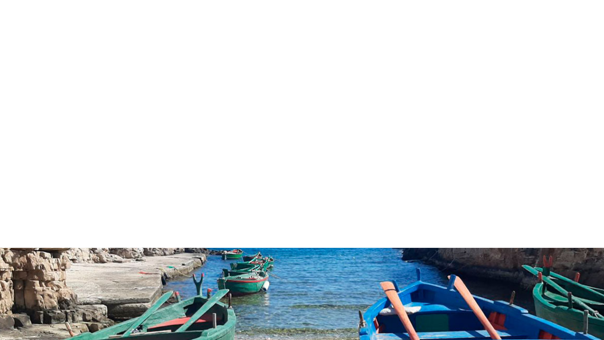
\includegraphics[width=\paperwidth]{background/template_169.pdf}}%
\begin{frame}[noframenumbering,plain]
  \begin{center}
    \setlength{\parskip}{0pt}
    \vspace{10pt}
    {\Huge\bf Survey Discussion}
  \end{center}
\end{frame}
}

{
\usebackgroundtemplate{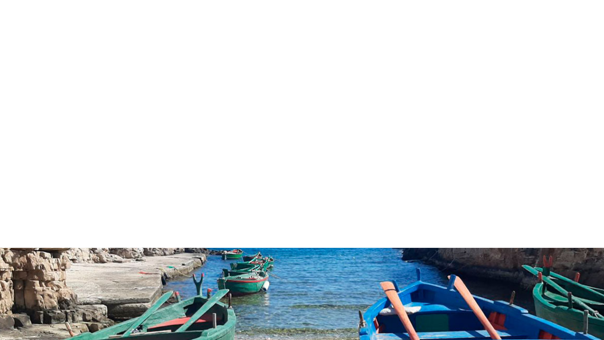
\includegraphics[width=\paperwidth]{background/template_169.pdf}}%
\begin{frame}[noframenumbering,plain]
  \begin{center}
    \setlength{\parskip}{0pt}
    \vspace{10pt}
    {\Huge\bf Wrap Up}
  \end{center}
\end{frame}
}

\begin{frame}
  \frametitle{\bf Where is our data from: CERN}
  \vspace{-5pt}
      \begin{figure}
        \includegraphics[width=0.90\textwidth]{figures/l3/cern.png}
      \end{figure}
\end{frame}

\begin{frame}
  \frametitle{\bf Where is our data from: CERN}
  \vspace{-5pt}
      \begin{figure}
        \includegraphics[width=0.90\textwidth]{figures/l3/cern_members.png}
      \end{figure}
      \blfootnote{Image copyright: 2012-2023 CERN}
\end{frame}

\begin{frame}[fragile]
  \frametitle{\bf Large Hadron Collider at CERN}
  \vspace{-5pt}
  \begin{figure}
    \includegraphics[width=0.90\textwidth]{figures/l1/intro/lhc_snip.png}
  \end{figure}
\end{frame}

\begin{frame}[fragile]
  \frametitle{\bf CERN OpenData}
  \vspace{-5pt}
  \begin{figure}
    \includegraphics[width=0.90\textwidth]{figures/l3/opendata.png}
  \end{figure}
\end{frame}

\begin{frame}[fragile]
  \frametitle{\bf ATLAS \Hgamgam{} dataset}
  \href{https://opendata.cern.ch/record/15006}{DOI:10.7483/OPENDATA.ATLAS.B5BJ.3SGS}
  \vspace{-5pt}
  \begin{figure}
    \includegraphics[width=0.90\textwidth]{figures/l3/atlas_gamgam.png}
  \end{figure}
\end{frame}

\begin{frame}[fragile]
  \frametitle{\bf ML datasets}
  \begin{itemize}
  \item LHC research involves complex detectors and 100-s of PB of data.
  \end{itemize}
  \begin{itemize}
\item ML is ubiquitous; data collection, analysis and simulation pipelines.
  \end{itemize}
  \begin{itemize}
  \item Several CERN Open Data datasets target machine learning.
  \end{itemize}
  \begin{itemize}
  \item Examples from the ATLAS collaboration:
  \begin{itemize}
    \item \href{https://opendata.cern.ch/record/15010}{\textcolor{EDBBlue}{Jet reconstruction training}}
    \item \href{https://opendata.cern.ch/record/15013}{\textcolor{EDBBlue}{Top Tagging}}
    \item
      \href{https://opendata.cern.ch/record/15012}{\textcolor{EDBBlue}{Generative
          Adversarial Network for detector simulation}}
    \item \href{https://opendata.cern.ch/record/328}{\textcolor{EDBBlue}{Higgs Boson Machine Learning Challenge}}
  \end{itemize}   
  \end{itemize}
\end{frame}

{
\usebackgroundtemplate{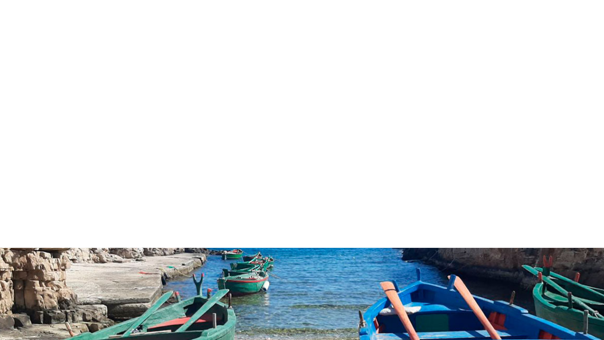
\includegraphics[width=\paperwidth]{background/template_169.pdf}}%
\begin{frame}[fragile]
  \frametitle{\bf Summary}
  \adjustbox{valign=t}{\begin{minipage}[t][0.55\textheight]{\linewidth}
      \vspace{10pt}
  In this tutorial you:
  \begin{itemize}
  \item (1) Wrote a fully connected network to classify Higgs boson events.
  \item (2) Assessed that this classification results in an undesired bias
    (\myy{} distribution). 
  \item (3) Learned about the {\bf adversarial neural network technique}, and
    used it to remove this bias.    
  \end{itemize}
  Hope what you've learned will be useful for your work.
  \begin{center}
    {\bf Thank you and well done!}
  \end{center}
    \end{minipage}}
  \adjustbox{valign=t}{\begin{minipage}[t][0.35\textheight]{\linewidth} 
  \end{minipage}}
\end{frame}
}


\end{document}
